\chapter[Diagnostics, Control Systems, and People]{Diagnostics, Control Systems, and People\label{ch7}}

Feynamn: "all things are mmade of atoms..."

% If, in some cataclysm, all of scientific knowledge were to be destroyed, and only one sentence passed on to the next generation of creatures, what statement would contain the most information in the fewest words? I believe it is the atomic hypothesis that all things are made of atoms — little particles that move around in perpetual motion, attracting each other when they are a little distance apart, but repelling upon being squeezed into one another. In that one sentence, you will see, there is an enormous amount of information about the world, if just a little imagination and thinking are applied.

\section{Introduction}
\label{sec7.1}
If civilization were to be wiped out and only a single statement could be left carved in stone for future scientists to use, as they rebuilt civilization and invented gravitational wave detectors to reach out into the universe, it would be this:\\

"Think carefully and holistically about your detector before building it such that no part is neglected as being too small or 'second order', yea, for even the mighty may be brought low by the loose baffle or the unforseen cross-coupling."

The interferometer commissioning process has taught us that we could improve our design process.\\

We could divide things into subsystems as done in the chapters of a book, 
but then to make them work together things do not factor nearly so neatly. Controllability is much more important than the last few percent of 
isolation or noise performance.\\

It is not wise to design for a single point in parameter space: if each 
part of the interferometer can only work when all other pieces are 
performing as designed, it becomes impossible to integrate.\\

Its the inverse of a Sherlock Holmes locked-room mystery story.


\section{Detector Diagnostics}
   - we need testpoints everywhere

\begin{itmemize}
\item high frequency noise measurements to diagnose laser noise
\item HOM resonances
\item mirror mode ringups
\item even more important for parametric instability control\cite{Matt:PI}
\item non-uniform optic absorption
\item time dependence of optical scattering
\item how close are the optics to the stops
\item THD of the force actuators
\item THD of the displacement sensors
\item strain release in vacuum system couples to IFO by scattered light
\item bursts of gas lead to transient phase noise in arm cavities
\end{itemize}

\section{LIGO Mirror Suspensions: A Design Example}

Important considerations in test mass suspension design\cite{SUS:2012, Aston:2012}:
\begin{itemize}
   \item Vibration isolation: nearly all of the seismic isolation in the GW detection band ($f > 5\,\rm Hz$)
     comes from the suspension. To fulfill this requirement, the mirror must be isolated by a 
     multi-stage pendulum~\cite{Beker:2011}.
    \item low suspension thermal noise and minimization of creep noise~\cite{Levin:2012ek, Gretarsson:2005gs}
    \item third priority is some thoughts on damping
    \item 4th priority is minimize damping noise
    \item should instead consider upconversion, control forces, gradual noise reduction, minimization of angular noise generation, etc. all together in holistic metric v. sensitivity and uptime.
    \item Future suspension will look different than the LIGO/Virgo style
\end{itemize}

\section{Digital Control Systems: A second example}

​\section{Control System Synthesis}
  1) LIGO/Virgo/GEO done by pre-1980 controls technology: pole/zero placement, SISO error signal minimization, by-eye estimates of loop stability
  2) Techniques for process and aircraft control use more global and MIMO synthesis techniques with general cost function minimization.
  3) Machine learning techniques can use nonlinear cost functions and account for rare, large excursions -> maximize uptime

In recent years, more sophisticated algorithms have been introduced to better control the vibration isolation
systems supporting the mirrors in the interferometer~\cite{Beker:2014, Driggers:2012fl, Ryan:FFW2012}

  4) Adaptive machines can explore non-intuitive noise cancelation techniques​
  5) The dynamical response of the interferometer is a combination of mechanical, opto-mechanical, and electronic feedback. Its a mistake to treat these on such unequal footings - the interferometer design ought to be done using global search methods (such as MCMC) in the same way that we do for BHBH parameter estimation.

\section{Most Surprising Noise Sources}
\begin{itemize}
\item Classic bilinear: beam spot motion makes upconversion. Well understood in the 90's.
\item Limiting noise in S1: seen, but not understood until S2.
\item Weak LO: limit in S3. Found by noticing harmonics in spectra. Same structure as S1 OL noise.
\item Multiple PDs: the signal is not the same.
\item RF AS PD: What's in the I-phase?
\end{itemize}


\subsection{Scattered Light}
The phenomenon of excess phase noise due to scattered light has been known about for decades~\cite{DanDewey} at least.

Due to imperfections in the optics, for example, a small fraction of the laser light escapes from the main interferometer beam path. This light then interacts with something (e.g. a piece of the vacuum system or some other suspended optic or beam baffle) and then recombines with the circulating laser field within the 
interferometer~\cite{Kip:Baffles, Ottaway:scatter, Virgo:scatter, Partha:scatter}. The recombination may occur at virtually any point within the system: inside of the Fabry-Perot arm cavities, at the beamsplitter, or even at the final photodetector which records the GW strain signal.

It is instructive to consider quantitatively the ampltidue of the noise for a few of these cases. A significant source of scatter for all of the long interferometers
\begin{align}
S_x = some scattering stuff
\end{align}


\section{Risk Register and Risk Reduction Research}
\begin{itemize}
\item Keep a list of risks.
\item Gather detector experts to update list periodically.
\item Rate risks: probability of occurrence, potential impact, cost to fix
\item Risk Breakdown Structure and Risk Management Tools
\end{itemize}

\begin{figure}[h]
\centering
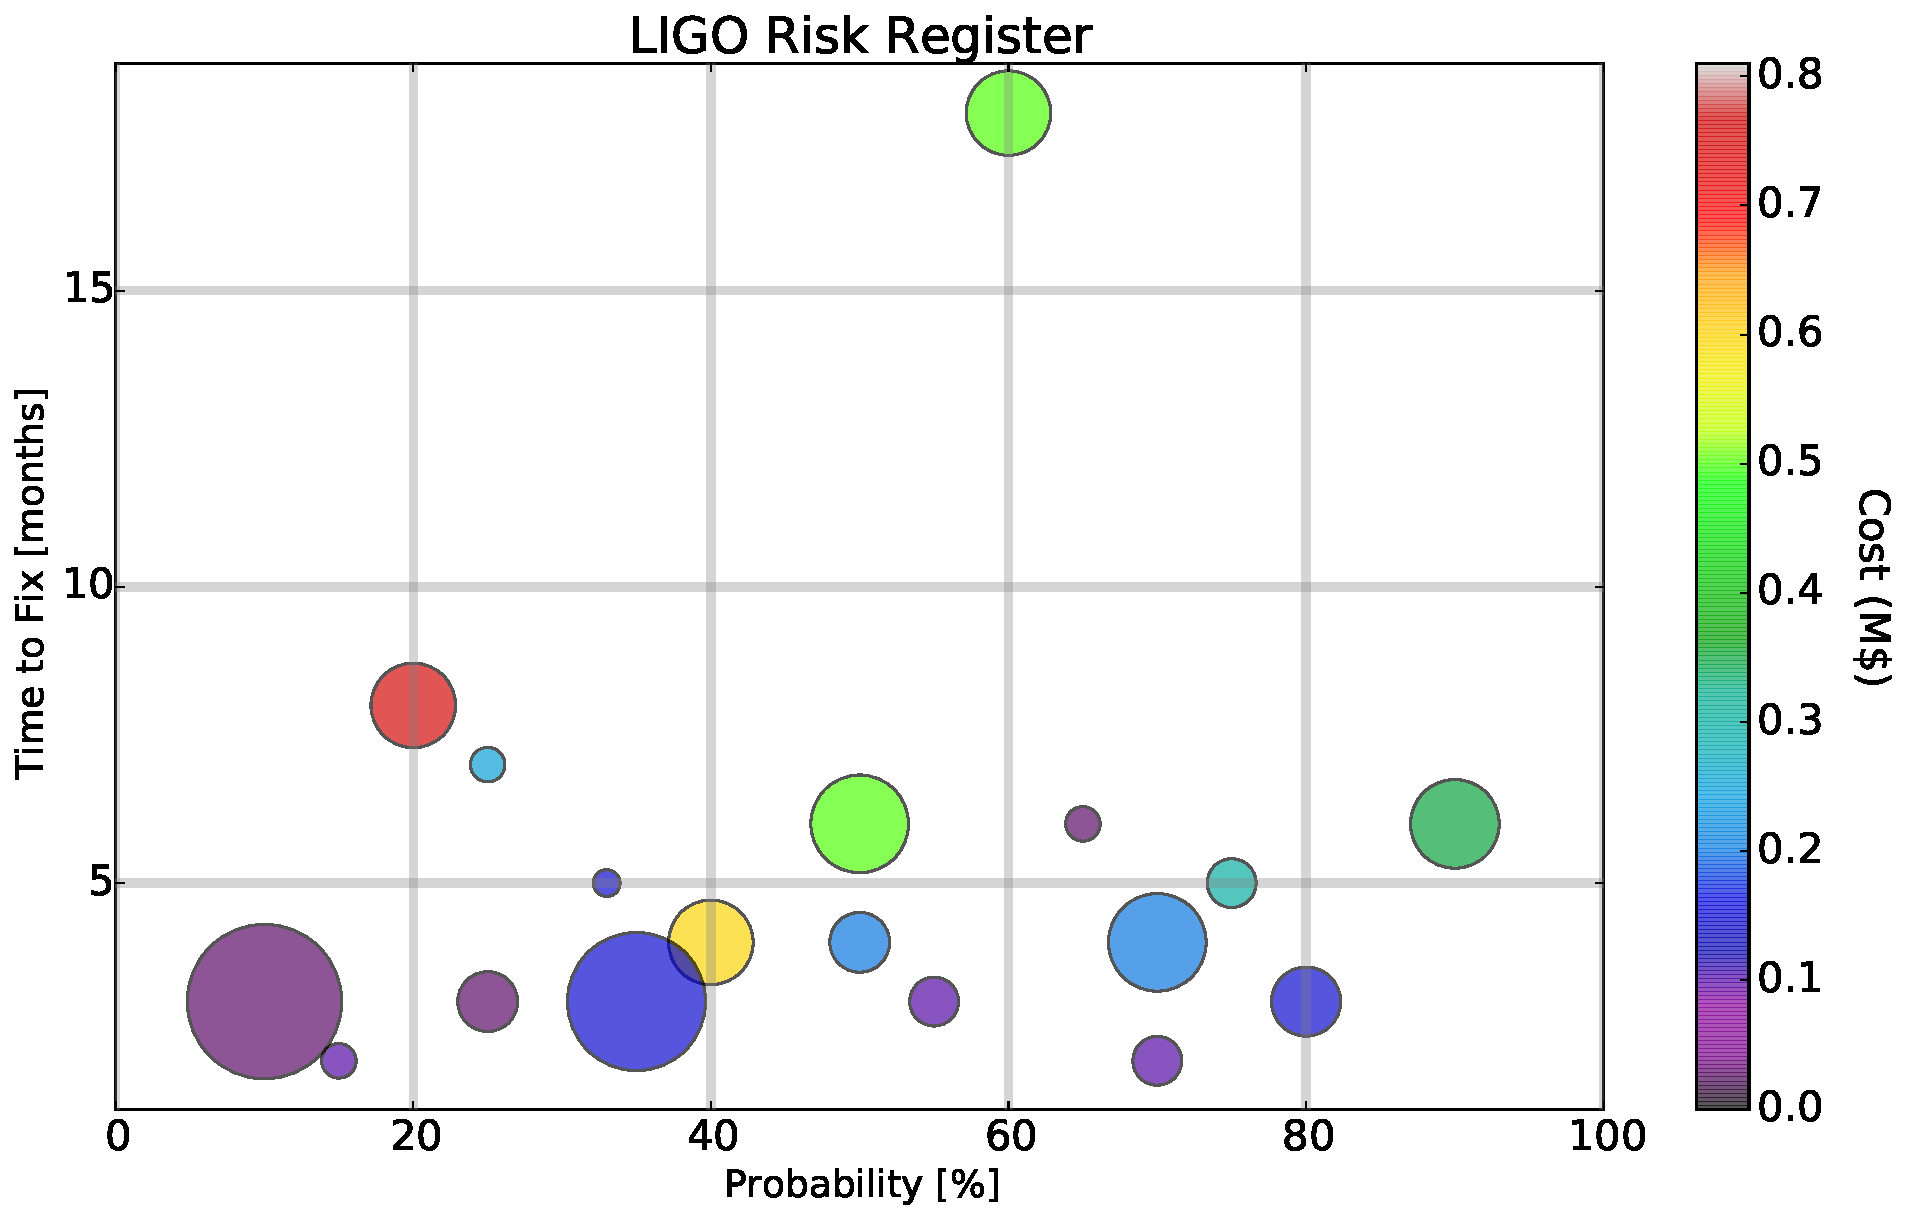
\includegraphics[width=\columnwidth]{Figures/Risk.pdf}
\caption{Risk Register for Advanced LIGO. Area of each circle represents the impact on the binary neutron star inspiral range.}
\label{fig:RiskBubbles}
\end{figure}


\section{People}
\begin{enumerate}
\item An important piece of the noise reduction feedback system 
  is the team of humans in the control room.
\item Viewed as a NN or ML algorithm, the machine needs to be 
  rewarded, punished, trained, and maintained in order to minimize 
  the time needed to reach the quantum sensitivity limits.
\item The team must also be able to train the next generation of machines.
\item In the Navy they teach the priority list of (1) complete the mission, 
  (2) safety, (3) train your replacement. How should we do this better?
\item How to balance making progress quickly and training the next 
  wave of young scientists?
\item The team needs to make progress quickly, but the PhD 
  students need theses and the local observatory staff need to 
  be fully engaged (not steamrolled) by visiting scientists 
  working 15 hour days.
\item Include some data here on grad students who did work on the
  interferometers (at CIT and MIT) and what they did next and where
  they are now. e.g., they stayed in the field N years, the left or not.
\end{enumerate}

\begin{figure}[h]
\centering
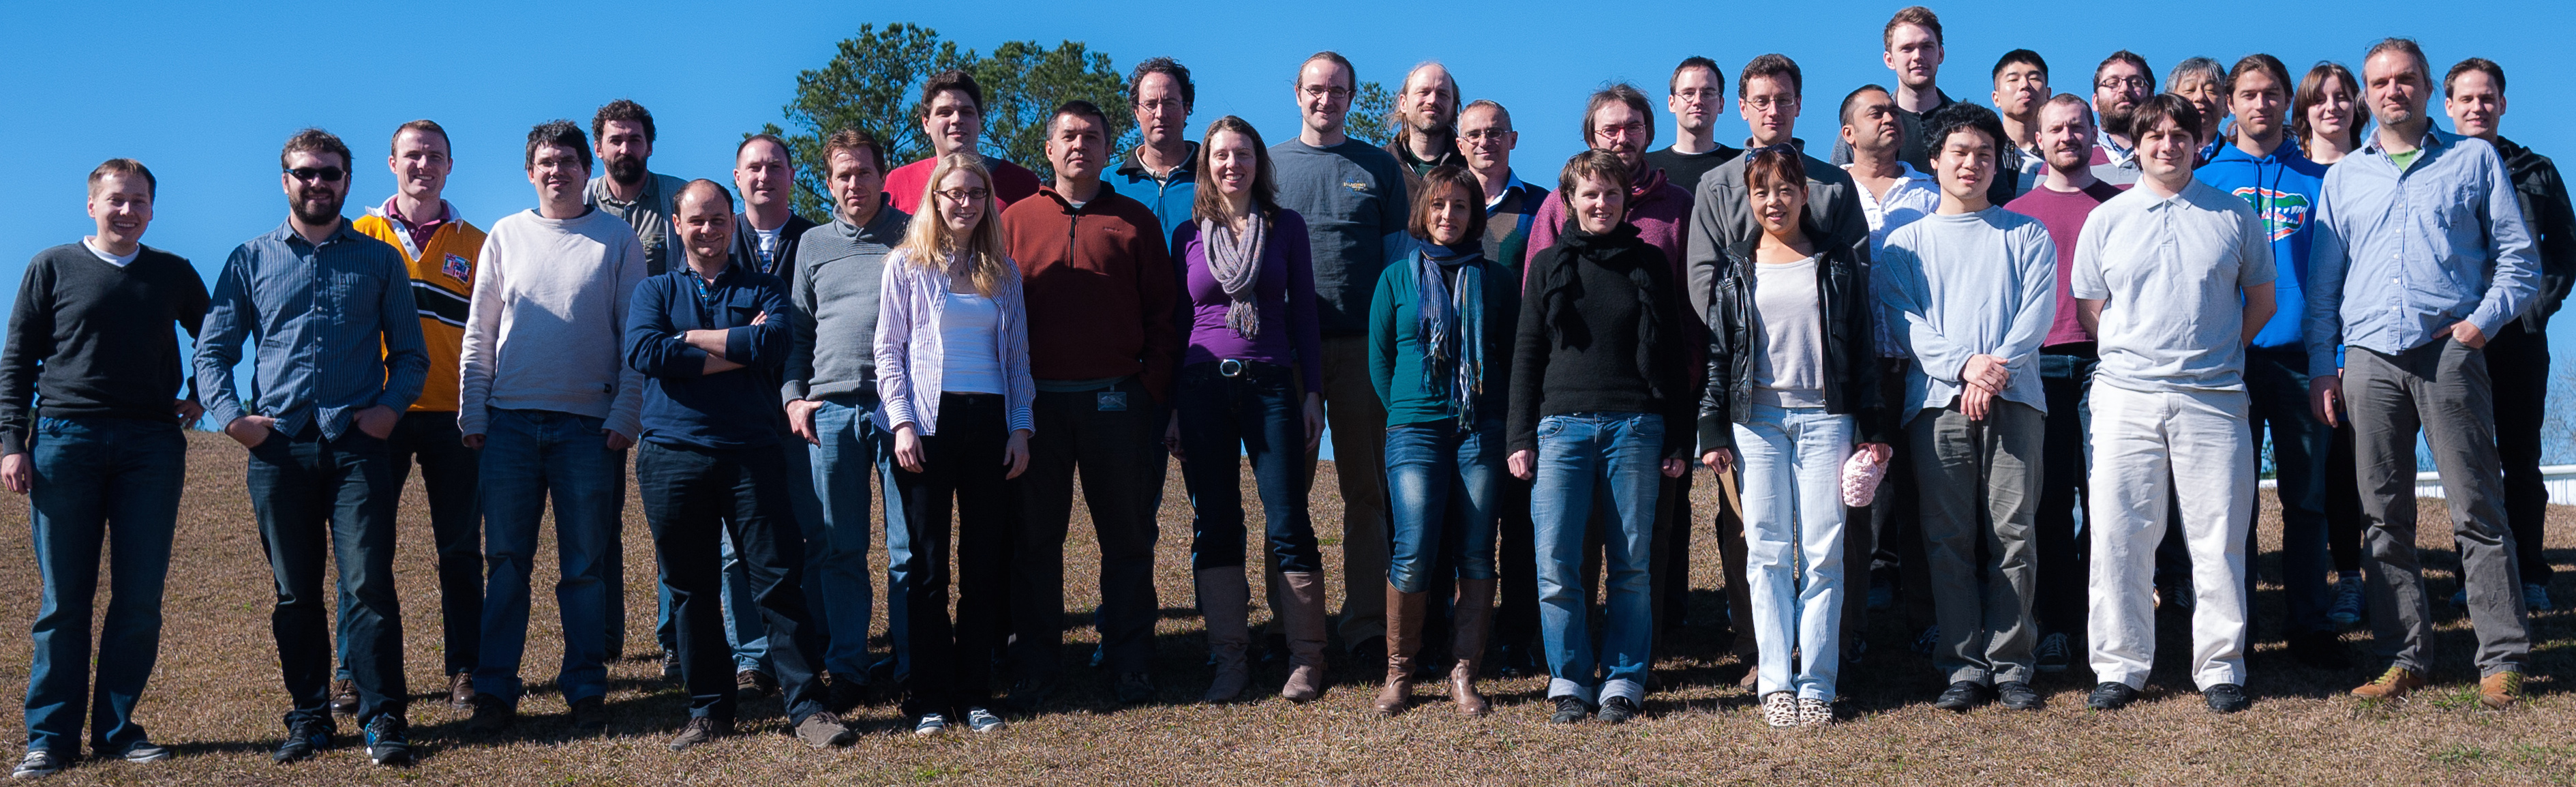
\includegraphics[width=\columnwidth]{Figures/GroupPhoto_LLOworkshop13.jpg}
\caption{International GW Commissioning workshop}
\label{fig:workshopPhotoLLO}
\end{figure}

\section{Conclusion}
These wise things should be kept in mind while doing the detector commissioning.

In addition to the usual thoughts about how to radically improve the detector sensitivity.



